\usetikzlibrary{positioning,arrows.meta,fit}
\begin{figure}[h]
  \centering
  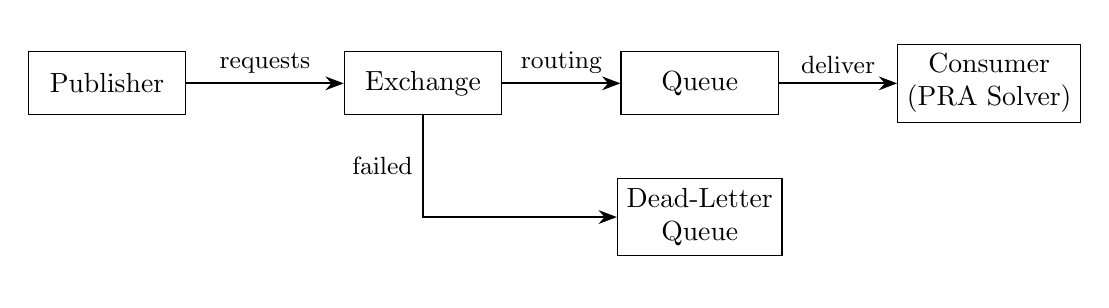
\begin{tikzpicture}[
      scale=0.7,
      >=Stealth,
      box/.style={draw,rectangle,minimum width=2cm,
                  minimum height=0.8cm,align=center},
      msg/.style={->, thick},
      label/.style={font=\small,draw=none}
    ]
    
    % Message Broker components
    \node[box] (exchange) {Exchange};
    \node[box, right=1.5cm of exchange] (queue) {Queue};
    \node[box, below=0.8cm of queue] (dlq) {Dead-Letter\\Queue};
    
    % Fit node for RabbitMQ Message Broker
    \node[fit=(exchange)(queue)(dlq),
          draw, inner sep=0.3cm, dashed, 
          label={[yshift=0.3cm]\textbf{RabbitMQ}}] (broker) {};
    
    % Publisher and Consumer
    \node[box, left=2cm of exchange] (publisher) {Publisher};
    \node[box, right=1.5cm of queue] (consumer) {Consumer\\(PRA Solver)};
    
    % Draw connections
    \draw[msg] (publisher) -- node[above,label]{requests} (exchange);
    \draw[msg] (exchange) -- node[above,label]{routing} (queue);
    \draw[msg] (queue) -- node[above,label]{deliver} (consumer);
    
    % Failed messages
    \draw[msg] (exchange) |- node[pos=0.25,left,label]{failed} (dlq);
    
  \end{tikzpicture}
  \caption{Publisher-consumer message flow with broker internals.}
  \label{fig:worker-pool-queue-management}
\end{figure}